\documentclass[reprint,amsmath,amssymb,aps, prl,superscriptaddress]{revtex4-2}
\usepackage{graphicx}% Include figure files
\usepackage{dcolumn}% Align table columns on decimal point
\usepackage{bm}% bold math
\usepackage{amsmath}
\usepackage{natbib}
\usepackage{chngcntr}
\usepackage{url}
\usepackage{float}
\usepackage{fourier} 
\usepackage{array}
\usepackage{makecell}
\usepackage{background}
\usepackage[english]{babel}
\usepackage[utf8]{inputenc}
\usepackage{fancyhdr}
\usepackage{physics}
\usepackage{subcaption}
\usepackage{titlesec}

\titleformat*{\subsection}{\large\bfseries}
\titleformat*{\section}{\Large\bfseries}
\pagestyle{fancy}
% \fancyhf{}
\rhead{Lab-C (TAU)}
\lhead{Quantum Cryptography}

\bibliographystyle{apsrev}

\setcounter{tocdepth}{5}
\setcounter{secnumdepth}{5}
\renewcommand\theadalign{bc}
\renewcommand\theadfont{\bfseries}
\renewcommand\theadgape{\Gape[4pt]}
\renewcommand\cellgape{\Gape[4pt]}
\backgroundsetup{
	scale=1,
	angle=0,
	opacity=1,
	color=black,
	contents={\begin{tikzpicture}[remember picture, overlay]
			\node at ([yshift = -1cm] current page.north)
			{
\includegraphics[width = 3cm]{Images/logo.png}}; %
	\end{tikzpicture}}
}
\begin{document}
\title{Using Quantum Mechanics For Secure Communication}
\author{Alon Shaaltiel}
\author{Oren Kereth}
\affiliation{Raymond and Beverly Sackler School of Physics and Astronomy, Faculty of Exact Sciences, Tel Aviv University, Tel Aviv 69978, Israel}
\author{Georgi Gary Rozenman}
\affiliation{Raymond and Beverly Sackler School of Physics and Astronomy, Faculty of Exact Sciences, Tel Aviv University, Tel Aviv 69978, Israel}
\affiliation{School of Electrical Engineering, Iby and Aladar Fleischman Faculty of Engineering, Tel Aviv University, Tel Aviv 69978, Israel}
\date{\today}
\begin{abstract}
Using linearly polarized light we execute the BB84 protocol
for quantum cryptography. The protocol is examined when no eavesdropper
is present and a key is transmitted securely between two users. The
results are compared with a simulation of the system. As the BB84
protocol uses quantum mechanics, an eavesdropper cannot measure the
signal without altering it and so they are detected. Detection of
an eavesdropper under the BB84 is also examined and the results are
compared with a simulation of the system.
\end{abstract}
\maketitle
\newcommand{\de}{^{\circ}}
\newcommand\Ket[1]{\ket{#1}}%
\renewcommand*{\thesection}{\arabic{section}}
\renewcommand*{\thesubsection}{\arabic{section}.\arabic{subsection}}
\part*{Introduction}

\section*{Historical Review}

The first documented use of cryptography is from Egypt dating 4000 years ago \cite{FirstdocumenteduseofCrypto}. Cryptography is the science of writing in secret code, which is necessary when communicating over any untrusted medium \cite{Cryptodorigins}. Most cryptographic protocols make use of ``keys'' to encrypt and decrypt data \cite{CryptoKeys}. The idea of quantum cryptography, which utilizes quantum mechanics in cryptographic protocols, was first proposed in the 1970s by Stephan Wiesner, Charles H.Bennet and Gilles Brassard \cite{QuantumCryptoOrigin}. Based on this idea, the protocol we use  in this experiment, BB84, was invented. BB84 allows its users to securely create an encryption key and to detect eavesdroppers \cite{ORIGINALBB84}. Since its invention, BB84 was proven to be secure both theoretically and experimentally \cite{BB84SECURETheory,BB84SECUREExperiment}. With the advancements of technology, practical implementations of BB84 are being tested. Among these implementations are satellite-to-ground quantum communication using BB84 encryption over a distance of 1200km \cite{BB84Satellite}, underwater communication\cite{BB84underwater1,BB84underwater2} and more. In the near future, BB84 could be used worldwide due to its secure nature and the improvement of technology over time. 

\section*{Theoretical Review}

A key that will  be used to encrypt data is formed from a sequence of '0's and '1's . In this experiment the polarization of light transmitted between the two communicating users, ``Alice'' and ``Bob'', is used to signify 0 and 1. The light can be polarized and measured in two different bases, $+$ and $\times$. In the $+$ basis, light can be linearly polarized at either $0\de$ or $90\de$, denoted by $\Ket{0\de}$ and $\Ket{90\de}$ respectively. These polarizations are by definition orthogonal  and therefore $\Ket{0\de}$ can denote '1' and $\Ket{90\de}$ can denote '0' without the two mixing. In the $\times$ basis, light can be polarized at either $45\de$ or $-45\de$, denoted similarly by $\Ket{45\de}$ and $\Ket{-45\de}$ respectively. These polarizations are orthogonal too, and so $\Ket{45\de}$ denotes '1' and $\Ket{-45\de}$ denotes '0' when the light is measured in this basis. Using linear algebra it can be shown that
\begin{equation}
\Ket{45\de}=\frac{1}{\sqrt{2}}(\Ket{0\de}+\Ket{90\de})\,;\Ket{-45\de}=\frac{1}{\sqrt{2}}(\Ket{0\de}-\Ket{90\de})\label{eq: Relation between X basis to + basis}
\end{equation}
 and similarly from these relations it can be shown that 
\begin{equation}
\Ket{0\de}=\frac{1}{\sqrt{2}}(\Ket{45\de}+\Ket{-45\de})\:;\Ket{90\de}=\frac{1}{\sqrt{2}}(\Ket{45\de}-\Ket{-45\de})\label{eq: Relation between + basis to X basis}
\end{equation}
Based on the quantum mechanical treatment of the polarizations, the
relations above indicate that measuring the polarization of light
that was polarized in the $\times$ basis in the $+$ basis has an
equal probability of yielding either '0' or '1', and vise-versa.

\subsection*{BB84}
The BB84 encryption protocol makes use of the two different bases that share the relations in equations \ref{eq: Relation between X basis to + basis} and \ref{eq: Relation between + basis to X basis}. The protocol is as follows: one of the communicating users, Alice, chooses a basis (either $+$ or $\times$) at random. Alice then chooses a bit in that basis (either 0 or 1) and transmits a photon with the corresponding polarization in the basis she has chosen. Independently, the second user, Bob, chooses a basis at which he measures the polarization of the transmitted photon. Upon measurement, Bob documents the result (either 0 or 1) and the basis at which he chose to measure the polarization, while Alice documents the basis and bit she chose to transmit. The two users repeat this step many times. Alice and Bob then go through their measurements and compare the bases they have chosen for each measurement. They then discard the measurements in which Alice and Bob have chosen different bases and keep only those that have the same basis. Alice and Bob then publicly compare bits from a sample group chosen at random from the remaining measurements. In an ideal communication channel that is not eavesdropped on, they expect all the bits to be the same (i.e if Alice sent a 1 in $\times$ basis and Bob chose to measure in the $\times$ basis he is guaranteed to get a 1 too) and thus from the remaining bits that they have not compared they will form the key with which they will now encrypt and decrypt data from each other. However, if there is an eavesdropper, ``Eve'', spying on their communication, she will inevitably interfere with the transmission, allowing us to intercept her.  Suppose Eve is eavesdropping on the communication between Alice and Bob. Eve receives the polarized photon from Alice. Suppose that Bob and Alice have both chosen the same basis in that measurement, $+$ and that Alice transmitted a 1. At a probability of $50\%$ Eve will choose the $+$ basis, leading to a correct measurement of the polarization. She will then replicate the result by choosing the basis with which she has measured the polarization, to transmit to Bob a photon polarized in that basis at a state corresponding to the bit she measured. In this case, she will transmit the exact same polarization to Bob, which will then receive exactly what Alice tried to transmit, leaving Eve undetected in this case. In the other $50\%$ of the cases, Eve will choose the wrong basis, $\times$. She will then transmit the photon with a polarization in that wrong basis, therefore, when Bob will measure the polarization in $50\%$ of the cases he will get a 1 and on the remaining $50\%$ of the cases he will get a 0. Therefore, despite choosing the exact same basis as Alice, in $50\%\times50\%=25\%$ of the cases he will measure the wrong bit because of Eve. Consequently, if $25\%$ of the compared bits turn out to be different from each other, Bob and Alice can detect Eve and cease communication on that channel. As we have shown here, BB84 allows its users to either detect an eavesdropper or to safely form a key with which they will communicate safely.

\subsection*{Half-Wave Plate}
As we have seen above, the protocol heavily relies on the ability of its users to transmit and measure photons with different polarizations. In this experiment this will be done using half-wave plates, also known as a ``polarization rotator''. A polarization rotator rotates the polarization of the incident light by double the physical rotation angle of the wave plate, denoted by $\theta$ (see Figure \ref{fig:Polarization Rotator Schematic}).

\begin{figure}[H]
	\centering
	\includegraphics[width=0.85\linewidth]{\string"Images/Polarization Rotator\string".jpg}
	\caption{A schematic of a polarization rotator. $\theta$ is the physical rotation
angle of the wave plate. Incident polarized light that passes through
the polarization rotator has its polarization rotated by $2\theta$.
\label{fig:Polarization Rotator Schematic}}
\end{figure}
 For example, if the incident light is in the state $\Ket{0\de}$
and the polarization rotator is rotated by $45\de$, the light will
be rotated to the $\Ket{90\de}$ state.

\part*{Experimental Setup}
The experiment consists of two parts. The first part contains only Alice and Bob communicating a key to each other without the existence of an eavesdropper on the channel. For the second part we add Eve, the eavesdropper. We then check if the BB84 protocol enables us to detect Eve.

\section*{First Part}
The experimental setup of the first part consists of two units. The first unit 'belongs' to Alice and is capable of transmitting light with different linear polarizations according to the two bases $+,\times$. The second unit belongs to Bob and is capable of detecting the light and measuring its polarization (see Figure \ref{fig: Experimental Setup - Part 1} ). 
\begin{figure}[H]
\includegraphics[width=\linewidth]{\string"Images/Experimental Setup - Part I\string".jpg}

\caption{The experimental setup of the first part. On the left- Alice's unit
which transmits the bits via polarized light. On the right- Bob's
unit which detects the light and measures its polarization. \label{fig: Experimental Setup - Part 1}}

\end{figure}
Alice's unit uses a single photon source  that produces vertically polarized light ($\Ket{0\de}$). The light then goes through a polarization rotator which can change the polarization of light to one of four angles at the two different bases: $+$ ($\Ket{0\de},\Ket{90\de}$) and $\times$ ($\Ket{45\de},\Ket{-45\de}$). In this method Alice is capable of transmitting bits of information in the two bases required for the protocol. Bob then chooses a basis of measurement by rotating the polarization of the incident light at either $0\de$ or $-45\de$. The polarized light then goes through a polarizing beamsplitter (PBS) that transmits the horizontal component of polarization ($\Ket{90\de})$ and reflects the vertical component ($\Ket{0\de}$). This  allows Bob to measure the polarization in the two different bases. For example, if Alice transmits $\Ket{45\de}$ (a 1 bit in the $\times$ basis) and Bob rotates the polarization by $-45\de$  (measuring in $\times$ basis) the light will turn to $\Ket{0\de}$. It will then be reflected by the PBS and Bob will measure a 1 as required. If Bob measures in the $+$ basis the polarization of the light will not change. Because $\Ket{45\de}$ consists of vertical and horizontal components in equal magnitude (according to equation \ref{eq: Relation between X basis to + basis}) half the time Bob will measure a 1 and in the other half he will measure a 0. We have thus shown that the composition of Bob's unit allows him to perform all the operations required of him according to the BB84 protocol. In this part of the experiment Alice sends to Bob three sequences of bits with varying lengths (18,50 and 100 bits), the bits that were sent and received with the same basis form the key, upon comparison we expect no errors as the system is ideal with no eavesdropper.

\section*{Second Part}
We now add an eavesdropper to the communication channel, Eve. Eve detects the photon transmitted by Alice and measures its bit in a randomly chosen basis. Eve then replicates the measured bit and transmits it to Bob in the same basis she measured in. To perform these operations according to the protocol, Eve's unit is a combination of Alice's and Bob's units (see Figure \ref{fig: Experimental Setup II }). 
\begin{figure}[H]
\includegraphics[width=\linewidth]{\string"Images/Experimental Setup - Part II\string".jpg}

\caption{The added unit to the experimental setup for the second part. Eve's
unit is a combination of Bob's and Alice's units. Eve is capable of
measuring bits from Alice and transmitting the results of her measurement
to Bob. \label{fig: Experimental Setup II }}

\end{figure} 
The ``Bob part'' of Eve's unit allows Eve to detect and measure the bits transmitted to her as explained in the first part and the ``Alice part' of Eve's unit allows her to transmit the measurement to Bob in the basis she has chosen. Apart from the addition of Eve to the setup nothing else has changed. In this part of the experiment we will attempt to detect Eve using the protocol with sequences of 18 bits, 50 bits and 100 bits.

\part*{Results}

\section*{First Part}
 By transmitting sequences of 18,50 and 100 bits from Alice to Bob, forming a key according to the protocol and comparing the results to a simulation the following results have been concluded (see Table
\ref{tab: Part I results table} ) 
\begin{table}[H]
	\centering
	\begin{tabular}{|c|c|c|}
		\hline 
		----------- & \thead{Experiment} & \thead{Simulation}\tabularnewline
		\hline 
		\hline 
		Sequence Length & \multicolumn{2}{c|}{Key Length($\%$ of bits)}\tabularnewline
		\hline 
		18 & 10(56\%) & 8(44\%)\tabularnewline
		\hline 
		50 & 27(54\%) & 27(54\%)\tabularnewline
		\hline 
		100 & 48(48\%) & 54(54\%)\tabularnewline
		\hline 
	\end{tabular}

\caption{First part - results table\label{tab: Part I results table}}

\end{table} 
As mentioned in a previous section, the length of the key is determined by the number of bits that were transmitted by Alice in the same basis as the one Bob used to measure them, leading to its correct interpretation (meaning that if Alice transmitted a '1' Bob also measured a '1'). According to our model, the probability Alice and Bob chose the same basis for a certain bit is $50\%$. In both the experiment and simulation it appears that the length of the key is close to the expectancy according to the model (which is half of the sequence length). Moreover, in the experiment and simulation all the bits that were measured and transmitted in the same basis by Bob and Alice respectively were correctly interpreted. This is exactly as the model predicts and as we require for the protocol to work (in its most ideal case, in reality communication errors can and will occur, but the protocol can still allow its users to deduct the existence of a spy). 

\section*{Second Part}
 After adding Eve to the setup as shown in \ref{fig: Experimental Setup II }, sequences of 18, 50 and 100 bits were transmitted from Alice to Bob and the results were analyzed according to the protocol. The bases for each bit measurement were compared and so were the bits corresponding to those measurements. From the comparison the following results have been concluded (see Table \ref{tab: Part II results table}) 
\begin{table}[H]
	\begin{subtable}[h]{0.45\textwidth}
		\centering
		\begin{tabular}{|c|c|c|} 
			\hline 
			\thead{Sequence Length} & \thead{\#SBBs ($\%$ of bits)} & \thead{\#Errors ($\%$ of bits)}\tabularnewline
			\hline 
			{18} & {8 (44\%)} & {2 (25\%)}\tabularnewline
			\hline 
			{50} & {18 (36\%)} & {3 (17\%)}\tabularnewline
			\hline 
			{100} & {54 (54\%)} & {13 (24\%)}\tabularnewline
			\hline 
		\end{tabular}
	\caption{Experimental results. SBBs stands for "same basis bits" (i.e. bits for which Alice and Bob chose the same basis for transmission and measurement).}
	\end{subtable}
	\begin{subtable}[h]{0.45\textwidth}
		\centering
		\begin{tabular}{|c|c|c|}
			\hline 
			\thead{Sequence Length} & \thead{\#SBBs($\%$ of bits)} & \thead{\#Errors ($\%$ of bits)}\tabularnewline
			\hline 
			{18} & {12 (66\%)} & {3 (25\%)}\tabularnewline
			\hline 
			{50} & {24 (48\%)} & {4 (17\%)}\tabularnewline
			\hline 
			{100} & {48 (48\%)} & {12 (25\%)}\tabularnewline
			\hline 
		\end{tabular}
	\caption{Simulation results. SBBs stands for "same basis bits".}
	\end{subtable}
\caption{Second part - experimental and simulation results. The percentage of errors was calculated according to the number of SBBs.\label{tab: Part II results table}}
\end{table} 

As the data shows, upon the insertion of Eve there are errors in SBBs (unlike the first part which had no errors). The percentages of errors for all sequence lengths are close to 25\% apart from the 17\% errors which was recorded for 50 bits. Figure \ref{fig: Simulation of the error as function of sequence length} shows the results from simulations of varying sequence lengths, for longer sequences the percentage of errors converges to 25\%, just as the model predicts. Also shown is the variance  in the percentage of errors around $x=50$. Assuming the distance from $25\%$ in each direction is three standard deviations away, the percentage around $x=50$ is $0.25_{-0.0700}^{+0.0972}$ (1$\sigma$ in each direction) which makes our measurement $1.1$ standard deviations away, well within the desired range.
\begin{figure}[H]
	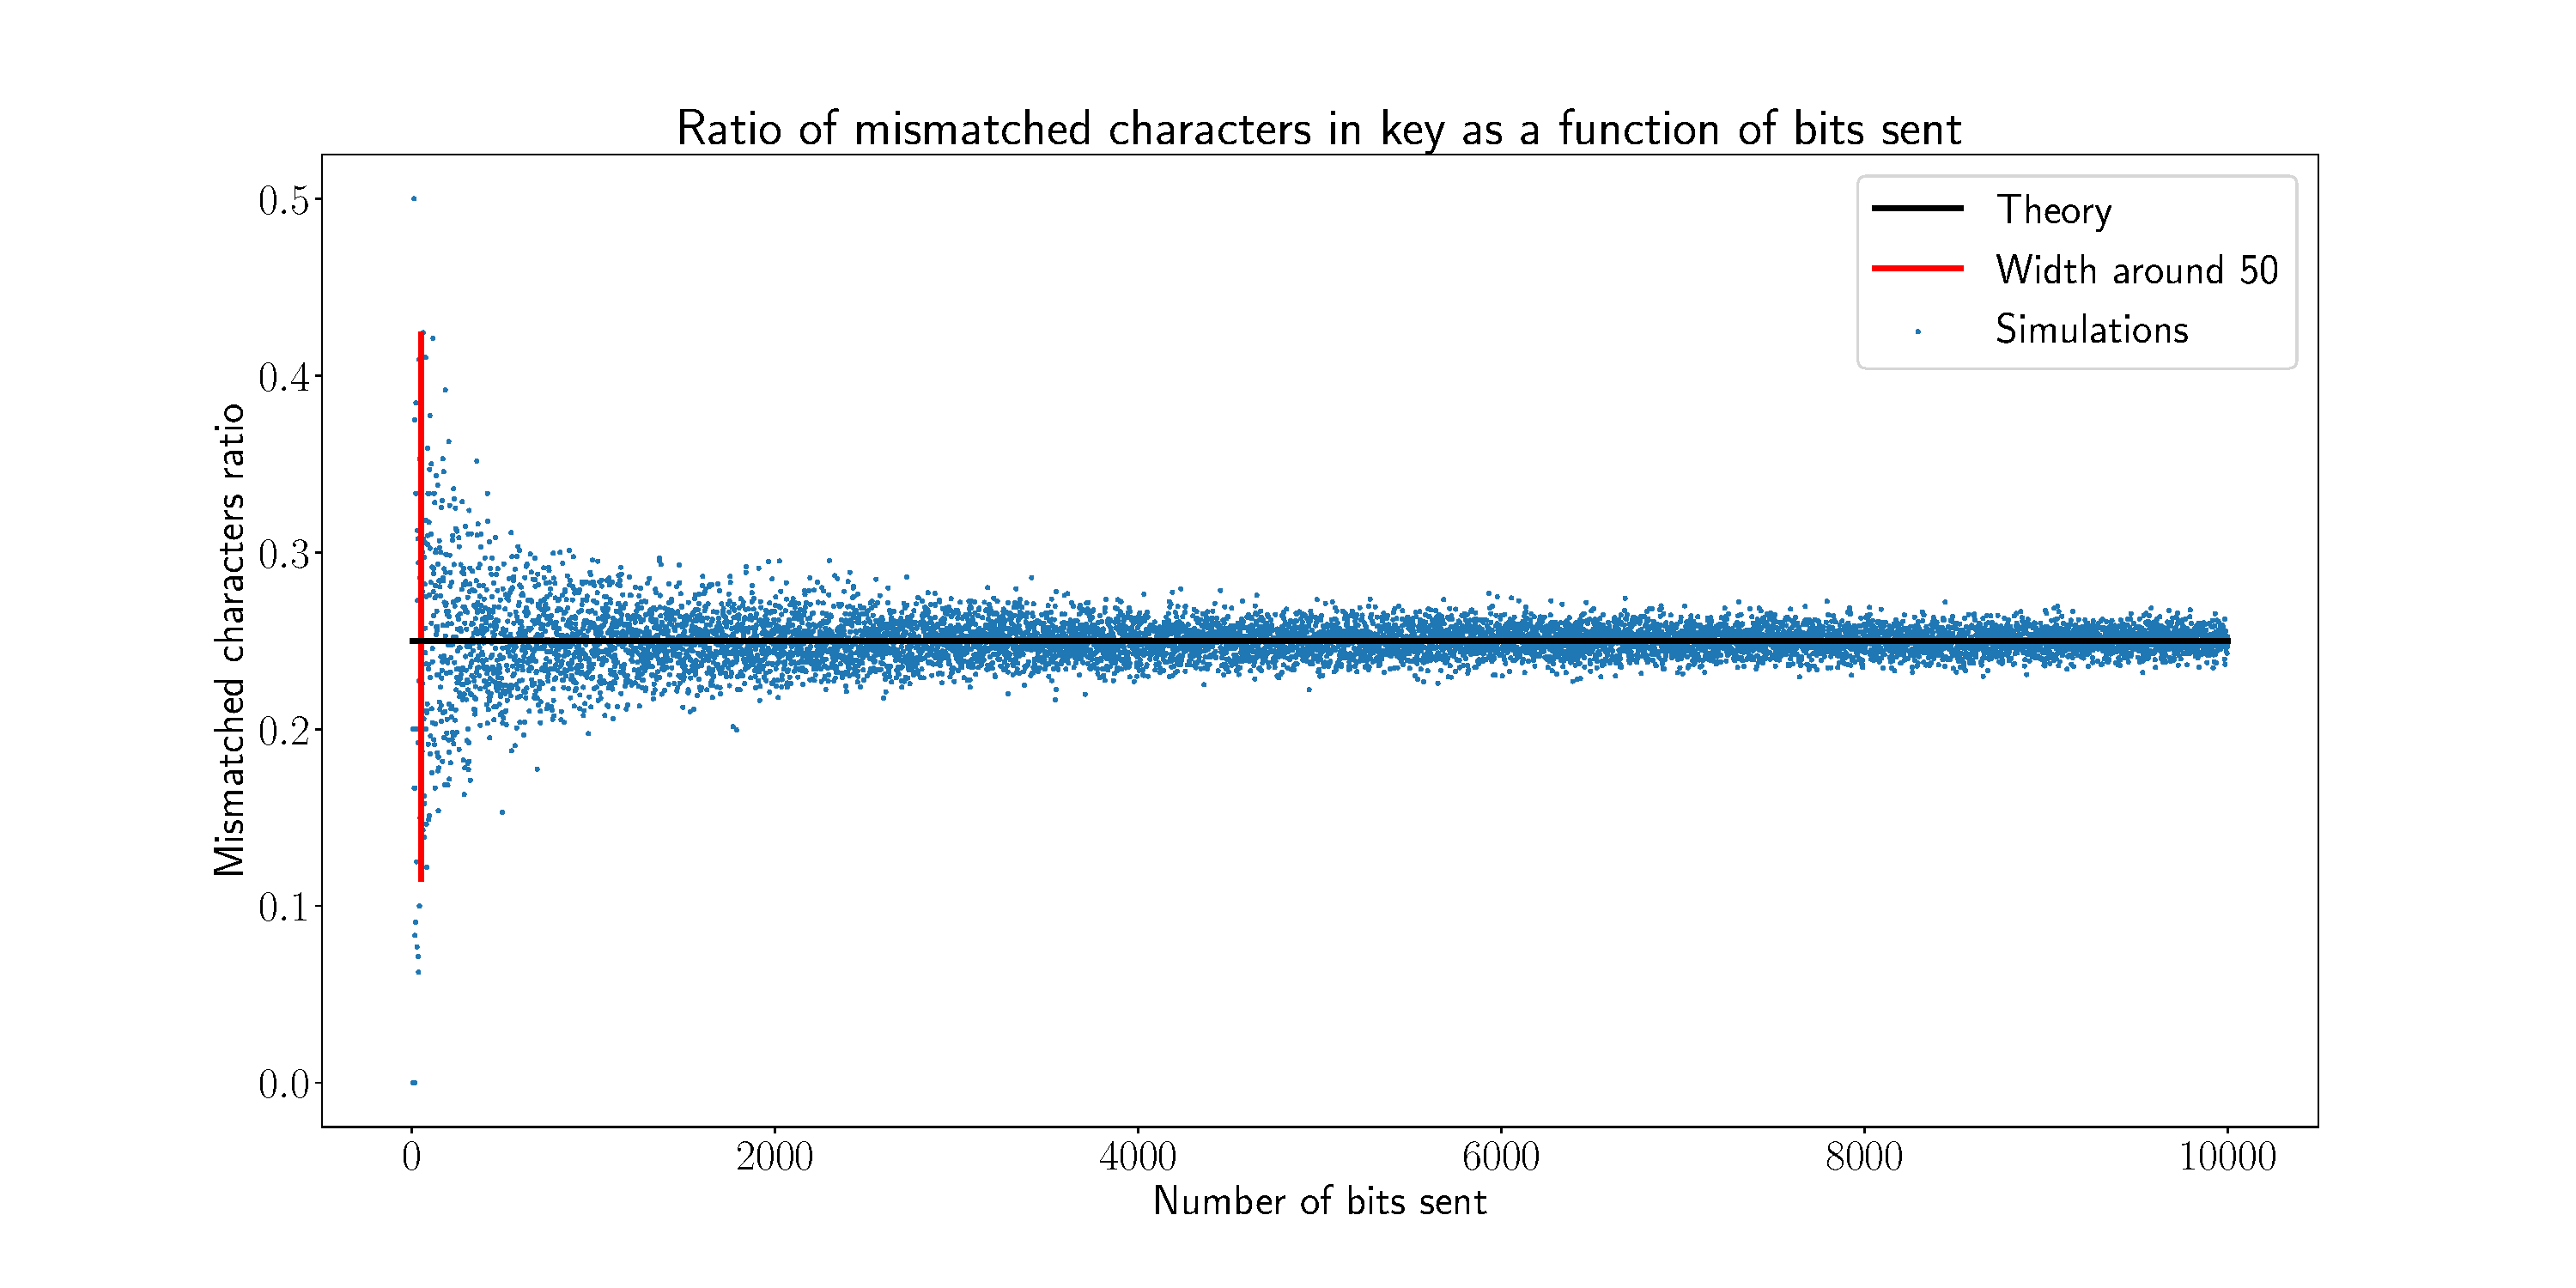
\includegraphics[width=\linewidth]{Images/PercentSimulation}

	\caption{Graph of the percentage of errors in SBBs. The blue dots are simulations, the red line around $x=50$ shows the width of the points around the black line at $y=0.25$, which is the theoretical value that the model predicts. \label{fig: Simulation of the error as function of sequence length}}
\end{figure}
Moreover, Figure \ref{fig: Binomial Distribution} shows that according to our model the probability of getting 3 errors for 18 SBBs (which led to the 17\% error for the 50 bits case) is greater than 5\% (more accurately it is about 17\%) and therefore the null hypothesis cannot be rejected and the model remains valid.
\begin{figure}[H]
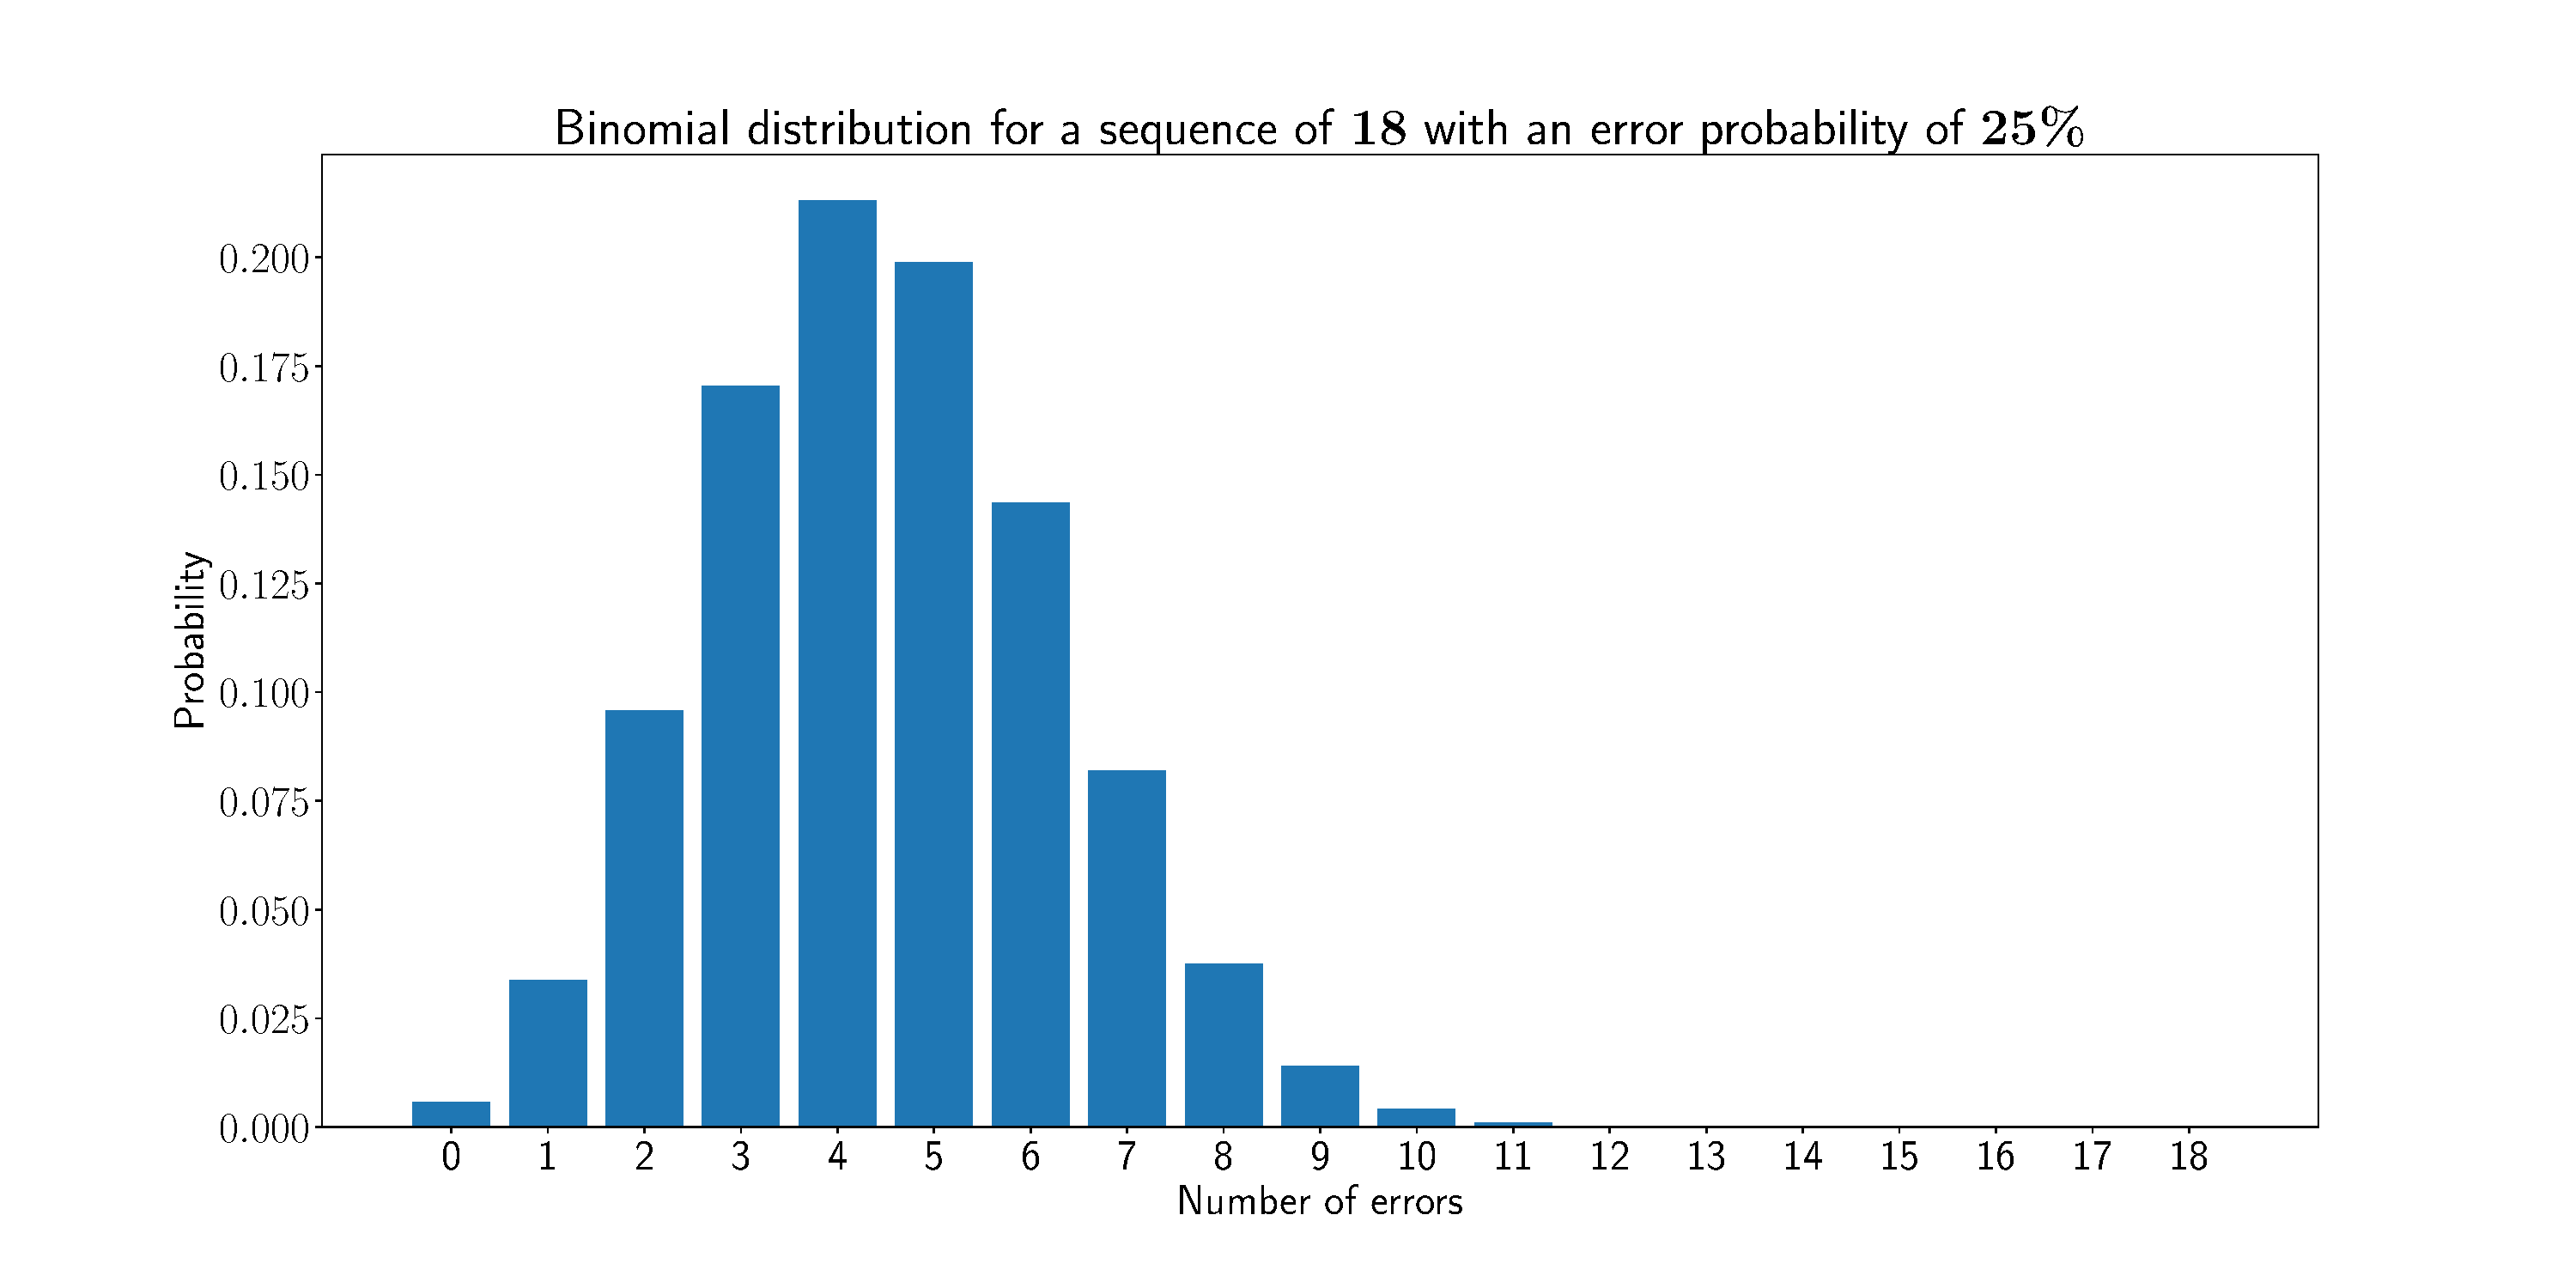
\includegraphics[width=\linewidth]{Images/BinomialDist18}

\caption{Binomial distribution for a sequence of 18 repetitions (18 SBBs) with a probability of 25\% to fail (probability of getting an error at a certain SBB). \label{fig: Binomial Distribution}}

\end{figure}
The BB84 protocol has therefore allowed us to detect Eve successfully.

\part*{Discussion}

In this experiment we communicated via the BB84 protocol. In the first part of the experiment there was no eavesdropper, which allowed Alice and Bob to form a key successfully according to the protocol. The key consisted of about half the bits transmitted, in accordance with our theoretical model. Moreover, no errors were spotted in the comparison of SBBs, yet again in accordance with theoretical results for the case of no eavesdropper. The simulation has also demonstrated similar results. In the second part an eavesdropper, Eve, was added. The BB84 protocol allowed us to detect Eve, because for all three sequences transmitted from Alice to Bob there were errors in the comparison of SBBs. For the sequence of 18 and 100 transmitted bits the percentage of errors compared to the number of SBBs was either 25\% or close to it. However, for the sequence of 50 bits the percentage was at about 17\%, which is not as close to 25\%. To assess this result, we used a binomial distribution whose probability of ``failure'' is 25\%, relying on the theoretical model. We have shown that the probability of getting three errors out out of 18 is greater than our set significance level of 5\%. In addition the expected variance in the ratio of errors was estimated using simulations and our measurement of 17\% is $1.1$ standard deviations from $25\%$ which is in the desired range of $3$ deviations. Therefore the theoretical model remains valid. We have also shown, using the simulation, that the percentage of errors converges to 25\% for longer and longer sequences of transmitted bits, just as the model predicts. The simulation demonstrated similar results that are, too, in agreement with the model. The results we have achieved are in accordance with a previous experiment examining the BB84 protocol. The experiment obtained a percentage of errors close to zero in the absence of an eavesdropper and a percentage close to 25\% in the presence of Eve \cite{9225317}. All in all, we have demonstrated that the BB84 protocol enables secure communication and that it's theoretical model is valid. 

\bibliographystyle{unsrt}
\bibliography{Report}

\end{document}
